\documentclass[a4paper,14pt,oneside,final]{extreport}

\usepackage[framemethod=default]{mdframed}
\usepackage{moreverb}

\usepackage{lastpage}
% Предоставляет проприетарный Times New Roman.
\usepackage{pscyr}

        % \usepackage[scaled=0.914]{XCharter}[2017/12/19] % Подключение русифицированных шрифтов XCharter

% Выбор шрифта по-умолчанию.
% Пункт 2.1.1 Требований по оформлению пояснительной записки.
% Примечание: В требованиях не указан, какой именно шрифт использовать. По традиции используем TNR.
\renewcommand{\rmdefault}{ftm}
% \renewcommand{\familydefault}{Times New Roman}
% Установка кодировки исходных файлов.
\usepackage[utf8]{inputenc}
% Учет особенностей различных языков.
\usepackage[russian, english]{babel}
% Выбор внутренней TeX кодировки.
% \usepackage[T1,T2A]{fontenc}
\usepackage{polyglossia,fontspec}
% \usepackage{xunicode}

\setmainlanguage[babelshorthands=true]{russian}
\setotherlanguage{english}

\setmonofont{Courier New}
\newfontfamily\cyrillicfonttt{Courier New}
\defaultfontfeatures{Ligatures=TeX}

\setmainfont{Times New Roman}
\newfontfamily\cyrillicfont{Times New Roman}
\setsansfont{Arial}
\newfontfamily\cyrillicfontsf{Arial}

% Если планируете использовать Times New Romans (ftm), то нужно будет установить пакет PSCyr.
% PSCyr на Linux: http://plumbum-blog.blogspot.ru/2010/11/pscyr-tex-live.html?showComment=1290219013107#c2607271373129816963 (придется вспомнить команды копирования в терминале). На Windows инструкцию найти достаточно легко, как и исполнить её.

% \setmainfont{Times New Roman}
% Делает результирующий PDF "searchable and copyable".
\usepackage{cmap}
% Чтобы можно было использовать русские буквы в формулах, но в случае использования предупреждать об этом.
\usepackage[warn]{mathtext}
% Зачем: Добавляет поддержу дополнительных размеров текста 8pt, 9pt, 10pt, 11pt, 12pt, 14pt, 17pt, and 20pt.
% Почему: Пункт 2.1.1 Требований по оформлению пояснительной записки.
\usepackage{extsizes}
% Зачем: Длинна, пимерно соответвующая 5 символам
% Почему: Требования содержат странное требование про отсупы в 5 символов (для немоноширинного шрифта :| )
\newlength{\fivecharsapprox}
\setlength{\fivecharsapprox}{5ex}
% Зачем: Добавляет отступы для абзацев.
% Почему: Пункт 2.1.3 Требований по оформлению пояснительной записки.
\usepackage{indentfirst}
\setlength{\parindent}{\fivecharsapprox} % Примерно соответсвует 5 символам.
% Зачем: Настраивает межстрочный интервал, для размещения 40 +/- 3 строки текста на странице.
% Почему: Пункт 2.1.1 Требований по оформлению пояснительной записки.
\usepackage[nodisplayskipstretch]{setspace}
\setstretch{1.1}
% Зачем: Отключает использование изменяемых межсловных пробелов.
% Почему: Так не принято делать в текстах на русском языке.
\frenchspacing
% Сброс счетчика сносок для каждой страницы
% Примечание: в "Требованиях по оформлению пояснительной записки" не указано, как нужно делать, но в других БГУИРовских докуметах рекомендуется нумерация отдельная для каждой страницы
\usepackage{perpage}
\MakePerPage{footnote}
% Добавляет скобку 1) к номеру сноски
% Пункты 2.9.2 и 2.9.1 Требований по оформлению пояснительной записки.
\makeatletter \def\@makefnmark{\hbox{\@textsuperscript{\normalfont\@thefnmark)}}} \makeatother
% Зачем: Расположение сносок внизу страницы
% Почему: Пункт 2.9.2 Требований по оформлению пояснительной записки.
\usepackage[bottom]{footmisc}
% Переопределяем стандартную нумерацию, т.к. в отчете будут только section и т.д. в терминологии TeX
\makeatletter \renewcommand{\thesection}{\arabic{section}} \makeatother
% Зачем: Пункты (в терминологии требований) в терминологии TeX subsubsection должны нумероваться
% Почему: Пункт 2.2.3 Требований по оформлению пояснительной записки.
\setcounter{secnumdepth}{3}
% Зачем: Настраивает отступ между таблицей с содержанимем и словом СОДЕРЖАНИЕ
% Почему: Пункт 2.2.7 Требований по оформлению пояснительной записки.
\usepackage{tocloft}
\setlength{\cftbeforetoctitleskip}{-1em}
\setlength{\cftaftertoctitleskip}{1em}
% Определяет отступы слева для записей в таблице содержания.
% Пункт 2.2.7 Требований по оформлению пояснительной записки.
\makeatletter
	\renewcommand{\l@section}{\@dottedtocline{1}{0.5em}{1.2em}}
	\renewcommand{\l@subsection}{\@dottedtocline{2}{1.7em}{2.0em}}
\makeatother
% Задает стиль заголовков раздела жирным шрифтом, прописными буквами, без точки в конце
% Пункты 2.1.1, 2.2.5, 2.2.6 и ПРИЛОЖЕНИЕ Л Требований по оформлению пояснительной записки.
\makeatletter
\renewcommand\section{%
  \clearpage\@startsection {section}{1}%
    {\fivecharsapprox}%
    {-1em \@plus -1ex \@minus -.2ex}%
    {1em \@plus .2ex}%
    {\hyphenpenalty=10000\normalfont\normalsize\bfseries\MakeUppercase}}
\makeatother


% Зачем: Задает стиль заголовков подразделов
% Почему: Пункты 2.1.1, 2.2.5 и ПРИЛОЖЕНИЕ Л Требований по оформлению пояснительной записки.
\makeatletter
\renewcommand\subsection{%
  \@startsection{subsection}{2}%
    {\fivecharsapprox}%
    {-1em \@plus -1ex \@minus -.2ex}%
    {1em \@plus .2ex}%
    {\raggedright\hyphenpenalty=10000\normalfont\normalsize\bfseries}}
\makeatother
% Зачем: Задает стиль заголовков пунктов
% Почему: Пункты 2.1.1, 2.2.5 и ПРИЛОЖЕНИЕ Л Требований по оформлению пояснительной записки.
\makeatletter
\renewcommand\subsubsection{
  \@startsection{subsubsection}{3}%
    {\fivecharsapprox}%
    {-1em \@plus -1ex \@minus -.2ex}%
    {1em \@plus .2ex}%
    {\raggedright\hyphenpenalty=10000\normalfont\normalsize\bfseries}}
\makeatother
% Зачем: для оформления введения и заключения, они должны быть выровнены по центру.
% Почему: Пункты 1.1.15 и 1.1.11 Требований по оформлению пояснительной записки.
\makeatletter
\newcommand\sectioncentered{%
  \clearpage\@startsection {section}{1}%
    {\z@}%
    {-1em \@plus -1ex \@minus -.2ex}%
    {1em \@plus .2ex}%
    {\centering\hyphenpenalty=10000\normalfont\normalsize\bfseries\MakeUppercase}%
    }
\makeatother
% Зачем: Задает стиль библиографии
% Почему: Пункт 2.8.6 Требований по оформлению пояснительной записки.
\bibliographystyle{ugost2008}
% Зачем: Пакет для вставки картинок
% Примечание: Объяснение, зачем final - http://tex.stackexchange.com/questions/11004/why-does-the-image-not-appear
\usepackage{graphicx}
% \DeclareGraphicsExtensions{.pdf,.png,.jpg,.eps}
% Зачем: Директория в которой будет происходить поиск картинок
\graphicspath{{.}}
% Зачем: Добавление подписей к рисункам
\usepackage[nooneline]{caption}
\usepackage{subcaption}
% Зачем: чтобы работала \No в новых латехах
\DeclareRobustCommand{\No}{\ifmmode{\nfss@text{\textnumero}}\else\textnumero\fi}
% Зачем: поворот ячеек таблиц на 90 градусов
\usepackage{rotating}
\DeclareRobustCommand{\povernut}[1]{\begin{sideways}{#1}\end{sideways}}
% Зачем: Задание подписей, разделителя и нумерации частей рисунков
% Почему: Пункт 2.5.5 Требований по оформлению пояснительной записки.
\DeclareCaptionLabelFormat{stbfigure}{Рисунок #2}
\DeclareCaptionLabelFormat{stbtable}{Таблица #2}
\DeclareCaptionLabelFormat{stblisting}{Листинг #2}
\DeclareCaptionLabelSeparator{stb}{~--~}
\captionsetup{labelsep=stb}
\captionsetup[figure]{labelformat=stbfigure,justification=centering}
\captionsetup[table]{labelformat=stbtable,justification=raggedright}
\captionsetup[listing]{labelformat=stblisting,justification=centering}

\newenvironment{longlisting}{\captionsetup{type=listing}}{}
% \captionsetup[listing]{labelformat=stblisting,justification=centering}
\renewcommand{\thesubfigure}{\asbuk{subfigure}}

% Зачем: Окружения для оформления формул
% Почему: Пункт 2.4.7 требований по оформлению пояснительной записки и специфические требования различных кафедр
% Пример использования смотри в course_content.tex, строка 5
\usepackage{calc}
\newlength{\lengthWordWhere}
\settowidth{\lengthWordWhere}{где}
\newenvironment{explanationx}
    {%
    %%% Следующие строки определяют специфические требования разных редакций стандартов. Раскоменнтируйте нужную строку
    %% стандартный абзац, СТП-01 2010
    %\begin{itemize}[leftmargin=0cm, itemindent=\parindent + \lengthWordWhere + \labelsep, labelsep=\labelsep]
    %% без отступа, СТП-01 2013
    \begin{itemize}[leftmargin=0cm, itemindent=\lengthWordWhere + \labelsep , labelsep=\labelsep]%
    \renewcommand\labelitemi{}%
    }
    {%
    %\\[\parsep]
    \end{itemize}
    }

% Старое окружение для "где". Сохранено для совместимости
\usepackage{tabularx}
\newenvironment{explanation}
    {
    %%% Следующие строки определяют специфические требования разных редакций стандартов. Раскоменнтируйте нужные 2 строки
    %% стандартный абзац, СТП-01 2010
    \par
    \tabularx{\textwidth-\fivecharsapprox}{@{}ll@{ --- } X }
    %% без отступа, СТП-01 2013
    %\noindent
    %\tabularx{\textwidth}{@{}ll@{ --- } X }
    }
    {
    \\[\parsep]
    \endtabularx
    }
% Зачем: Удобная вёрстка многострочных формул, масштабирующийся текст в формулах, формулы в рамках и др
\usepackage{amsmath}
% Зачем: Поддержка ажурного и готического шрифтов
\usepackage{amsfonts}
% Зачем: amsfonts + несколько сотен дополнительных математических символов
\usepackage{amssymb}
% Зачем: Окружения «теорема», «лемма»
\usepackage{amsthm}
% Зачем: Производить арифметические операции во время компиляции TeX файла
\usepackage{calc}
% Зачем: Производить арифметические операции во время компиляции TeX файла
\usepackage{fp}
% Зачем: Пакет для работы с перечислениями
 \usepackage{enumitem}
 \makeatletter \AddEnumerateCounter{\asbuk}{\@asbuk}{щ)} \makeatother
% Зачем: Устанавливает символ начала простого перечисления
% Почему: Пункт 2.3.5 Требований по оформлению пояснительной записки.
 \setlist{nolistsep}
% Зачем: Устанавливает символ начала именованного перечисления
% Почему: Пункт 2.3.8 Требований по оформлению пояснительной записки.
\renewcommand{\labelenumi}{\asbuk{enumi})}
\renewcommand{\labelenumii}{\arabic{enumii})}
% Зачем: Устанавливает отступ от границы документа до символа списка, чтобы этот отступ равнялся отступу параграфа
% Почему: Пункт 2.3.5 Требований по оформлению пояснительной записки.
\setlist[itemize,0]{itemindent=\parindent + 2.2ex,leftmargin=0ex,label=--}
\setlist[enumerate,1]{itemindent=\parindent + 2.7ex,leftmargin=0ex}
\setlist[enumerate,2]{itemindent=\parindent + \parindent - 2.7ex}
% Зачем: Дополнительные возможности в форматировании таблиц
\usepackage{makecell}
\usepackage{multirow}
\usepackage{array}
% Зачем: "Умная" запятая в математических формулах. В дробных числах не добавляет пробел
% Почему: В требованиях не нашел, но в русском языке для дробных чисел используется {,} а не {.}
\usepackage{icomma}
% Зачем: макрос для печати римских чисел
\makeatletter
\newcommand{\rmnum}[1]{\romannumeral #1}
\newcommand{\Rmnum}[1]{\expandafter\@slowromancap\romannumeral #1@}
\makeatother
% Зачем: Управление выводом чисел.
\usepackage{sistyle}
\SIdecimalsign{,}
% Зачем: inline-коментирование содержимого.
\newcommand{\ignore}[2]{\hspace{0in}#2}
% Зачем: Возможность коментировать большие участки документа
\usepackage{verbatim}
\usepackage{xcolor}
% Зачем: Оформление листингов кода
% Примечание: final нужен для переопределения режима draft, в котором листинги не выводятся в документ.
\usepackage[final]{listings}
\usepackage[normalem]{ulem}

\usepackage{url}
\usepackage[final,hidelinks]{hyperref}
% Моноширинный шрифт выглядит визуально больше, чем пропорциональный шрифт, если их размеры одинаковы. Искусственно уменьшаем размер ссылок.
\renewcommand{\UrlFont}{\footnotesize\rmfamily\tt}

\usepackage[square,numbers,sort&compress]{natbib}
\setlength{\bibsep}{0em}

% Магия для подсчета разнообразных объектов в документе
\usepackage{lastpage}
\usepackage{totcount}
\regtotcounter{section}

\usepackage{etoolbox}

\newcounter{totfigures}
\newcounter{tottables}
\newcounter{totreferences}
\newcounter{totequation}

\providecommand\totfig{}
\providecommand\tottab{}
\providecommand\totref{}
\providecommand\toteq{}

\makeatletter
\AtEndDocument{%
  \addtocounter{totfigures}{\value{figure}}%
  \addtocounter{tottables}{\value{table}}%
  \addtocounter{totequation}{\value{equation}}
  \immediate\write\@mainaux{%
    \string\gdef\string\totfig{\number\value{totfigures}}%
    \string\gdef\string\tottab{\number\value{tottables}}%
    \string\gdef\string\totref{\number\value{totreferences}}%
    \string\gdef\string\toteq{\number\value{totequation}}%
  }%
}
\makeatother

\pretocmd{\section}{\addtocounter{totfigures}{\value{figure}}\setcounter{figure}{0}}{}{}
\pretocmd{\section}{\addtocounter{tottables}{\value{table}}\setcounter{table}{0}}{}{}
\pretocmd{\section}{\addtocounter{totequation}{\value{equation}}\setcounter{equation}{0}}{}{}
\pretocmd{\bibitem}{\addtocounter{totreferences}{1}}{}{}

% Для оформления таблиц не влязящих на 1 страницу
\usepackage{longtable}

% Для включения pdf документов в результирующий файл
\usepackage{pdfpages}
% Для использования знака градуса и других знаков
% http://ctan.org/pkg/gensymb
\usepackage{gensymb}
% Зачем: преобразовывать текст в верхний регистр командой MakeTextUppercase
\usepackage{textcase}
% Зачем: Переносы в словах с тире.
% Тире в словае заменяем на \hyph: аппаратно\hyphпрограммный.
% https://stackoverflow.com/questions/2193307/how-to-get-latex-to-hyphenate-a-word-that-contains-a-dash#
\def\hyph{-\penalty0\hskip0pt\relax}
\usepackage{amsmath}
\usepackage{amsfonts}
\usepackage{amssymb}
\usepackage{graphicx}
\usepackage{lmodern}
\usepackage{float}
% поля
\usepackage[a4paper,left=30mm,right=10mm,top=20mm,bottom=20mm,nohead,nofoot,nomarginpar]{geometry}
% толерантность к переносам
\tolerance 6000%
% для списка источников
\makeatletter \renewcommand{\@biblabel}[1]{\stepcounter{totreferences}#1 \hfill} \makeatother
% для случая, когда документ маленький, и всего одна секция
%\renewcommand{\thesection}{}
%\renewcommand{\thesubsection}{\arabic{subsection}}
%\renewcommand{\thesubsubsection}{\arabic{subsection}.\arabic{subsubsection}}
% не помню зачем. Кажется, разреживает таблицу.
\renewcommand{\arraystretch}{1.5}

\renewcommand{\rmdefault}{cmr} % Шрифт с засечками
\renewcommand{\sfdefault}{cmss} % Шрифт без засечек
\renewcommand{\ttdefault}{cmtt} % Моноширинный шрифт
\renewcommand{\labelitemi}{--}
\renewcommand{\labelenumi}{\theenumi.}

\usepackage{chngcntr}
\counterwithin{equation}{section}

\usepackage{indentfirst}
\usepackage{cool}
\usepackage{commath}

\newcommand*\rfrac[2]{{}^{#1}\!/_{#2}}
\DeclareMathAlphabet{\mathpzc}{OT1}{pzc}{m}{it}
\newcommand{\z}{\mathpzc{z}}
\usepackage{mathtools}

\usepackage{hyperref}
\hypersetup{colorlinks = true}
% для правильной и быстрой записи дифференциалов и частных производных
\usepackage{physics}
\allowdisplaybreaks
%\displaybreak[0]
% http://tex.stackexchange.com/questions/42271/floor-and-ceiling-functions
\usepackage{mathtools}
\DeclarePairedDelimiter{\ceil}{\lceil}{\rceil}

\usepackage{amsmath}
\usepackage{tcolorbox}

\usepackage{listings}

\usepackage{color}
\definecolor{dkgreen}{rgb}{0,0.6,0}
\definecolor{gray}{rgb}{0.5,0.5,0.5}
\definecolor{mauve}{rgb}{0.58,0,0.82}
\definecolor{deepblue}{rgb}{0,0,0.5}
\definecolor{deepred}{rgb}{0.6,0,0}
\definecolor{deepgreen}{rgb}{0,0.5,0}

% Default settings for code listings
\lstset{frame=tb,
  aboveskip=3mm,
  belowskip=3mm,
  showstringspaces=false,
  columns=flexible,
  basicstyle=\renewcommand{\baselinestretch}{0.95}\ttfamily,
  numbers=none,
  numberstyle=\tiny\color{gray},
  keywordstyle=\bfseries\color{orange!40!black},
  commentstyle=\itshape\color{purple!40!black},
  identifierstyle=\color{black},
  emph={Main,MyMath, Data, Solution,
  		Int, Double, String, Array, Unit,
  		Console, math},          % Custom highlighting
  emphstyle = \color{deepgreen},    % Custom highlighting style
  stringstyle=\color{mauve},
  frame=L,
  xleftmargin=\parindent,
  breaklines=true,
  breakatwhitespace=true
  tabsize=3
  framexleftmargin=8mm,
  rulesepcolor=\color{blue},
}

\usepackage{minted}
\usepackage{xcolor}
\colorlet{LightGray}{black!5!}
\setminted[cpp]{fontsize=\footnotesize,tabsize=2,breaklines=true,bgcolor=LightGray}

\usepackage{tikz}
\usepackage{pgfplots}
% We will externalize the figures
\usepgfplotslibrary{external}
\tikzexternalize

\usepackage{cleveref}

\begin{document}
  \begin{titlepage}
    \begin{center}
      \small
      МИНИСТЕРСТВО НАУКИ И ВЫСШЕГО ОБРАЗОВАНИЯ РОССИЙСКОЙ ФЕДЕРАЦИИ \\
      ФЕДЕРАЛЬНОЕ ГОСУДАРСТВЕННОЕ БЮДЖЕТНОЕ ОБРАЗОВАТЕЛЬНОЕ УЧРЕЖДЕНИЕ ВЫСШЕГО ОБРАЗОВАНИЯ \\
      \guillemotleft НОВОСИБИРСКИЙ ГОСУДАРСТВЕННЫЙ ТЕХНИЧЕСКИЙ УНИВЕРСИТЕТ\guillemotright \\
      \normalsize
      Кафедра вычислительной техники \\

      \vspace{12em}
      % \includegraphics[width=3cm]{nstu_logo}
      % \vspace{3em}

      \textbf{Отчет по лабораторным работам \textnumero 1-6 \\
      по дисциплине: \guillemotleft Программирование\guillemotright \\}
    \end{center}
    \vspace{5em}
    \begin{tabular}{ll}
      Факультет:     & АВТФ \\
      Группа:        & АВТ-143\\
      Студент:       & Васютин А.\,М. \\
      Преподаватель: & Новицкая Ю.\,В. \\
      Вариант:       & 4 \\
    \end{tabular}
    \vspace{\fill}
    \begin{center}
      Новосибирск, 2022 г. \\
    \end{center}
  \end{titlepage}


  \newpage
  \renewcommand\contentsname{\centerline{\bfseries\normalsize{\MakeUppercase{Оглавление}}}}
  \normalsize\selectfont
  \tableofcontents

  \newpage\section{Лабораторная работа \textnumero 1. Разработка классов, создание конструкторов и деструкторов}
  \subsection{Цель работы}
  \par Изучить структуру класса, механизм создания и использования, описание членов-данных класса и методов доступа к ним, возможность инициализации объектов класса с помощью конструкторов и уничтожение их с помощью деструкторов.
  \subsection{Задание на лабораторную работу}
  \par Реализовать класс в соответствии с вариантом. Класс должен обеспечивать набор методов для работы с данными. Создать перегруженные конструкторы: конструктор с параметрами, конструктор копирования, конструктор по умолчанию.
  \par Реализовать указанные классы с динамическим выделением памяти для хранения некоторых полей. Создать деструктор для освобождения памяти. Посмотреть в отладчике, как вызываются конструкторы и деструкторы.
  \par Составить демонстрационную программу. Для реализации демонстрационной программы использовать отдельный модуль. Программу построить с использованием проекта (см. файл «Пример проекта С++.docx»). Посмотреть работу программы в отладчике, обратить внимание на представление данных. Построить программу без отладочной информации. Обратить внимание на размер программы.
  \par Построить класс для работы с квадратными матрицами. Класс должен включать соответствующие поля: порядок, набор коэффициентов (динамическое выделение памяти для набора коэффициентов).
  \par Класс должен обеспечивать простейшие функции для работы с данными класса: транспонирование матрицы, вывод матрицы в удобной форме, сложение двух объектов класса.

  \subsection{Решение}
  \par Класс в языке C++ -- это пользовательский тип, класс определяется ключевым словом \textit{class} и сопутствующим синтаксисом. Класс может включать поля (статические и нестатические, включая битовые поля), методы (статические и нестатические), вложенные типы (классы, энумерации, синонимы существующих типов), а так же шаблоны членов и шаблоны переменных (начиная с c++14).

  \par У матрицы было создано 3 поля -- размеры матрицы и указатель на массив коэффициентов матрицы, были реализованы конструкторы и деструкторы (листинги\ref{lst:matrix-hpp1} и \ref{lst:matrix-cpp1}). Так же были реализованы методы \textit{transpose}, \textit{plus}, \textit{fprint} и \textit{print}.

  \begin{figure}[H]\centering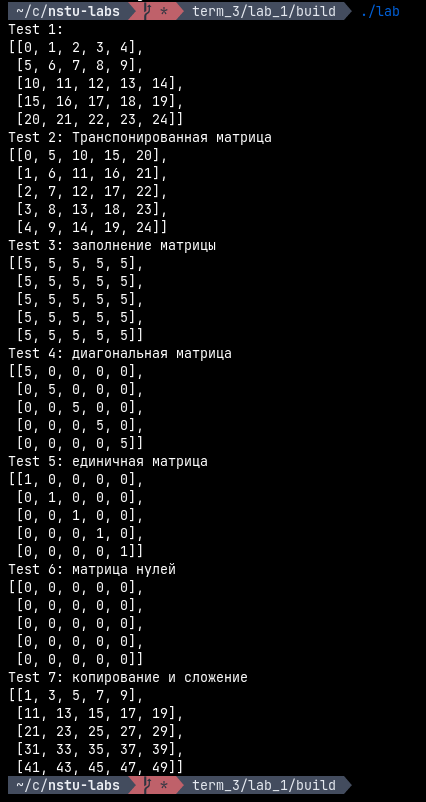
\includegraphics[width=0.5\textwidth]{lab1-test}\label{fig:lab1-test}\caption{Вывод работы программы.}\end{figure}

  \subsection{Исходный код}
  \begin{longlisting}\caption{main.cpp}\inputminted{cpp}{../../lab_1/main.cpp}\label{lst:main-cpp1}\end{longlisting}
  \begin{longlisting}\caption{matrix.hpp}\inputminted{cpp}{../../lab_1/matrix.hpp}\label{lst:matrix-hpp1}\end{longlisting}
  \begin{longlisting}\caption{matrix.cpp}\inputminted{cpp}{../../lab_1/matrix.cpp}\label{lst:matrix-cpp1}\end{longlisting}

  \subsection{Выводы}
  \par В ходе лабораторной работы были изучены базовые конструкции языка, связанные с классами. Были реализованы методы создания и разрушения объектов, а так же искомые методы. В реализациии работы был применен один из ключевых механизмов объектно-ориентированного программирования -- инкапсуляция, объединение данных и функций (методов), работающих с ними. Так же лабораторная работа состоит из нескольких файлов, следовательно, были отработаны навыки работы с многофайловыми проектами на языке C++.


  \newpage\section{Лабораторная работа \textnumero 2. Переопределение операций}
  \subsection{Цель работы}
  \par Ознакомиться с особенностями использования дружественных классов и функций, а также возможностью получения законченного нового типа данных, определив для него допустимые операции с помощью перегрузки операторов.Изучить структуру класса, механизм создания и использования, описание членов-данных класса и методов доступа к ним, возможность инициализации объектов класса с помощью конструкторов и уничтожение их с помощью деструкторов.
  \subsection{Задание на лабораторную работу}
  \par Для разработанного класса из лабораторной работы №1 реализовать набор операций для работы с объектами класса: сложение (как метод класса), вычитание (как дружественную функцию), присваивание (как метод класса), инкремент постфиксный и инкремент префиксный (как методы класса) (разобраться и вникнуть, в чем между ними разница!), приведение к некоторому типу (как метод класса).
  \par Дополнить демонстрационную программу, продемонстрировав все перегруженные операции.
  \subsection{Решение}

  \par Механизмы перегрузки операторов с языке c++ позволяют пользовательским типам мимикрировать под встроенные типы или же расширять функционал пользовательских типов используя привычный синтаксис его использования.

  \par Для класса были реализованы основные арифметические операции, а так же оператор \textit{()} для двух аргументов, что позволяет создать удобный интерфейс получения значения или ссылки определенного коэффициента матрицы. Префиксный и постфиксный инкременты и декременты синтаксически отличаются наличием у постфиксных операторов аргумента. Префиксный оператор сначала проводит инкрементирование объекта и возвращает его, а постфиксный оператор создает копию объекта, инкрементирует его и возвращает копию, следовательно, операции производимые с объектом, который был вернут постфиксным инкрементом не изменяют исходный объект, т.к. он является отдельным объектом.

  \begin{figure}[H]\centering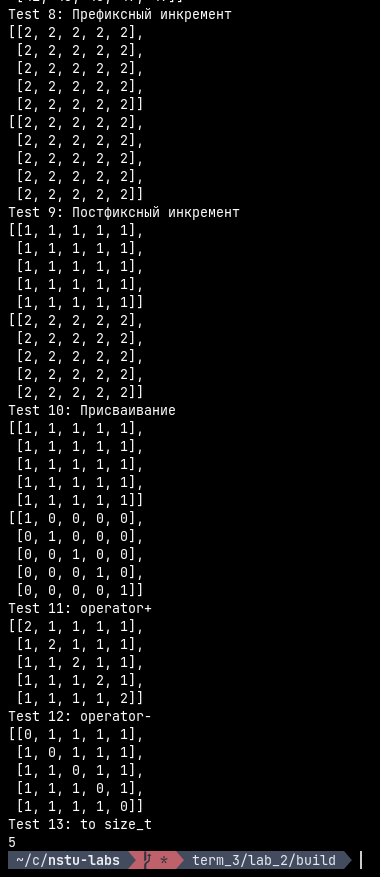
\includegraphics[width=0.5\textwidth]{lab2-test}\label{fig:lab2-test}\caption{Вывод работы программы.}\end{figure}

  \subsection{Исходный код}
  \begin{longlisting}\caption{main.cpp}\inputminted{cpp}{../../lab_2/main.cpp}\label{lst:main-cpp2}\end{longlisting}
  \begin{longlisting}\caption{matrix.hpp}\inputminted{cpp}{../../lab_2/matrix.hpp}\label{lst:matrix-hpp2}\end{longlisting}
  \begin{longlisting}\caption{matrix.cpp}\inputminted{cpp}{../../lab_2/matrix.cpp}\label{lst:matrix-cpp2}\end{longlisting}

  \subsection{Выводы}
  \par В ходе лабораторной работы были изучены механизмы перегрузки операторов, что позволяет переопределить поведение привычных операций для пользовательских типов, что позволяет увеличить читаемость кода в случае соответствия семантик оператора и переопределения, например, конкатенация строк.

  \newpage\section{Лабораторная работа \textnumero 3. Организация ввода-вывода}
  \subsection{Цель работы}
  \par Изучить работу потоков ввода-вывода и реализацию перегрузки потоков ввода-вывода на стандартные устройства и в файл для разработанных классов.
  \subsection{Задание на лабораторную работу}
  \par Для класса из лабораторной работы №2 перегрузить операции ввода/вывода, позволяющие осуществлять ввод и вывод в удобной форме объектов классов:
  \begin{itemize}
    \item вывод объекта класса в текстовый файл;
    \item вывод объекта класса в двоичный файл;
    \item ввод объекта класса из двоичного файла.
  \end{itemize}

  \par Дополнить демонстрационную программу, продемонстрировав все перегруженные операции.
  \subsection{Решение}

  \par Для работы с файлами был создан класс File, который является фасадом для объекта \textit{std::fstream}, а так же реализованы перегрузки оператора левого и правого сдвига (\textit{<<} и \textit{>>})


  \begin{figure}[H]\centering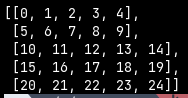
\includegraphics[width=0.5\textwidth]{lab3-test}\label{fig:lab3-test}\caption{Вывод работы программы.}\end{figure}
  \begin{figure}[H]\centering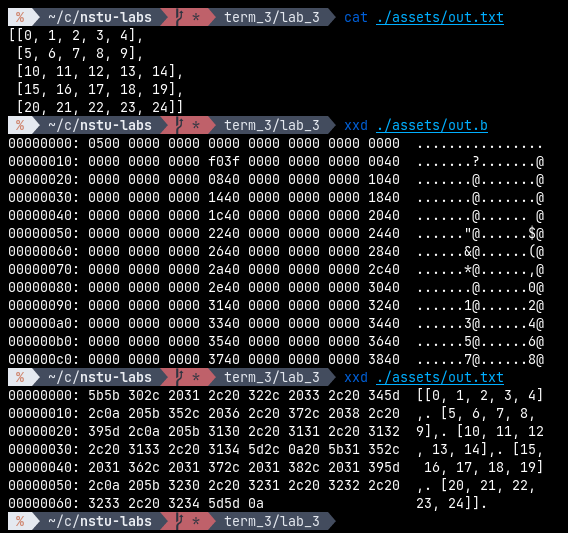
\includegraphics[width=0.9\textwidth]{lab3-files}\label{fig:lab3-files}\caption{Полученные файлы (\textit{in.b} -- копия \textit{out.b} ).}\end{figure}

  \subsection{Исходный код}
  \begin{longlisting}\caption{main.cpp}\inputminted{cpp}{../../lab_3/main.cpp}\label{lst:main-cpp3}\end{longlisting}
  \begin{longlisting}\caption{matrix.hpp}\inputminted{cpp}{../../lab_3/matrix.hpp}\label{lst:matrix-hpp3}\end{longlisting}
  \begin{longlisting}\caption{matrix.cpp}\inputminted{cpp}{../../lab_3/matrix.cpp}\label{lst:matrix-cpp3}\end{longlisting}
  \begin{longlisting}\caption{file.hpp}\inputminted{cpp}{../../lab_3/file.hpp}\label{lst:file-hpp3}\end{longlisting}
  \begin{longlisting}\caption{file.cpp}\inputminted{cpp}{../../lab_3/file.cpp}\label{lst:file-cpp3}\end{longlisting}

  \subsection{Выводы}
  \par В ходе лабораторной работы были изучены механизмы работы с файлами в языке c++, что является важной частью работы с данными.


  \newpage\section{Лабораторная работа \textnumero 4. Наследование}
  \subsection{Цель работы}
  \par Изучить механизм наследования и возможности порождения новых типов данных на основе уже существующих классов, изучить определение виртуальных функций и их использование для позднего связывания.
  \subsection{Задание на лабораторную работу}
  \par Для классов предыдущей лабораторной работы реализовать иерархию, изменяя отдельные методы и добавляя члены-данные (по усмотрению студента и преподавателя). В иерархию должно входить 2 производных класса. Один из методов должен быть виртуальным.
  \par Дополнить демонстрационную программу так, чтобы она демонстрировала создание, копирование объектов родственных типов, работу виртуальных функций.

  \subsection{Решение}

  \par Наследование -- один из механизмов объектно-ориентированного программирования, позволяющих создавая на основе каких либо классов производные, что убирает потребность в повторе кода и облегчает поддержку кода. В этой лабораторной работе была переработана структура классов, был создан базовый класс, представляющий матицу, и имеющий 3 наследника -- квадратную матрицу и 2 вектора (вертикальный и горизонтальный).
  \par Также был реплизован механизм виртуальных функций на основе метода \textit{fprint}. Таким образом, был реализован еще один механизм объектно-ориентированного программирования -- полиморфизм. Объекты типов с виртуальными функциями могут вызывая одни и те же функции получать их разное поведение (если вызывать их у указателя или ссылки на объект базового класса, но не значения), что показано в лабораторной работе (вектор печатается иначе).


  \begin{figure}[H]\centering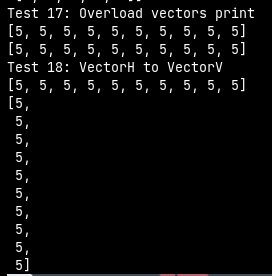
\includegraphics[width=0.5\textwidth]{lab4-test}\label{fig:lab4-test}\caption{Вывод работы программы.}\end{figure}

  \subsection{Исходный код}
  \begin{longlisting}\caption{main.cpp}\inputminted{cpp}{../../lab_4/main.cpp}\label{lst:main-cpp4}\end{longlisting}
  \begin{longlisting}\caption{matrix.hpp}\inputminted{cpp}{../../lab_4/matrix.hpp}\label{lst:matrix-hpp4}\end{longlisting}
  \begin{longlisting}\caption{matrix.cpp}\inputminted{cpp}{../../lab_4/matrix.cpp}\label{lst:matrix-cpp4}\end{longlisting}
  \begin{longlisting}\caption{file.hpp}\inputminted{cpp}{../../lab_4/file.hpp}\label{lst:file-hpp4}\end{longlisting}
  \begin{longlisting}\caption{file.cpp}\inputminted{cpp}{../../lab_4/file.cpp}\label{lst:file-cpp4}\end{longlisting}

  \subsection{Выводы}
  \par В данной работе был рассмотрены принципы объектно-ориентированного программирования: наследование и полиморфизм, получены знания о виртуальных функциях, позднем связывании и табице виртуальных функций (\textit{vtable}).


  \newpage\section{Лабораторная работа \textnumero 5. Создание динамического списка объектов, связанных наследованием}
  \subsection{Цель работы}
  \par Изучить работу с динамическими списочными структурами данных.
  \subsection{Задание на лабораторную работу}
  \par Реализовать с помощью классов динамическую списочную структуру, содержащую объекты классов, связанных наследованием. В классах реализовать методы добавления, удаления, вставки по номеру, удаления по номеру, поиска и просмотра всей структуры.
  \par Дополнить демонстрационную программу так, чтобы она демонстрировала полиморфическое поведение классов. Исследовать, как реализуется механизм полиморфизма.
  \par Структура данных: циклическая очередь, реализованная на двунаправленном списке.
  \par Способ хранения объектов: ссылки на объекты.
  \subsection{Решение}

  Циклическая очередь реализуется как класс \textit{CircularQueueOfMatrix}, хранящий указтель на первый элемент (ноду) \textit{CircularQueueOfMatrixNode}, которая в свою очередь хранит указатели на предыдущий и следующий элементы, а так же ссылку на матрицу.

  \begin{figure}[H]\centering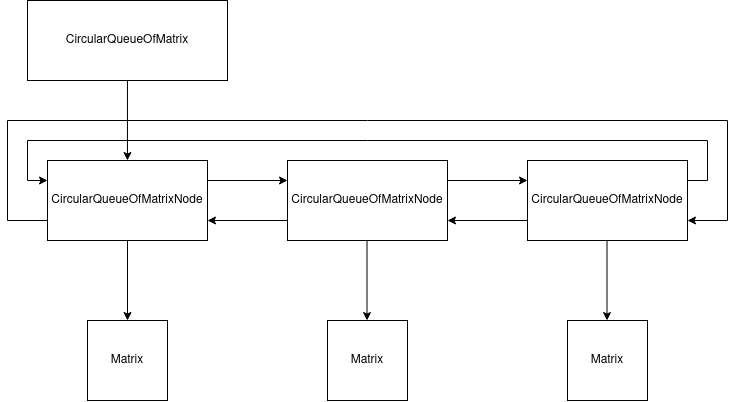
\includegraphics[width=\textwidth]{lab5-diagram}\label{fig:lab5-diagram}\caption{Рисунок организации циклической очереди.}\end{figure}
  \begin{figure}[H]\centering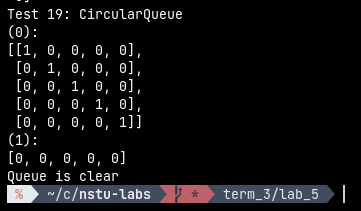
\includegraphics[width=0.5\textwidth]{lab5-test}\label{fig:lab5-test}\caption{Вывод работы программы.}\end{figure}

  \subsection{Исходный код}
  \begin{longlisting}\caption{main.cpp}\inputminted{cpp}{../../lab_5/main.cpp}\label{lst:main-cpp5}\end{longlisting}
  \begin{longlisting}\caption{matrix.hpp}\inputminted{cpp}{../../lab_5/matrix.hpp}\label{lst:matrix-hpp5}\end{longlisting}
  \begin{longlisting}\caption{matrix.cpp}\inputminted{cpp}{../../lab_5/matrix.cpp}\label{lst:matrix-cpp5}\end{longlisting}
  \begin{longlisting}\caption{file.hpp}\inputminted{cpp}{../../lab_5/file.hpp}\label{lst:file-hpp5}\end{longlisting}
  \begin{longlisting}\caption{file.cpp}\inputminted{cpp}{../../lab_5/file.cpp}\label{lst:file-cpp5}\end{longlisting}
  \begin{longlisting}\caption{circularqueue.hpp}\inputminted{cpp}{../../lab_5/circularqueue.hpp}\label{lst:circularqueue-hpp5}\end{longlisting}
  \begin{longlisting}\caption{circularqueue.cpp}\inputminted{cpp}{../../lab_5/circularqueue.cpp}\label{lst:circularqueue-cpp5}\end{longlisting}

  \subsection{Выводы}
  В этой лабораторной работе мы познакомились с разработкой полиморфных структор данных, при создании которых необходимо четко выделять интерфейсы для правильного обобщения хранимых в них типов.

  \newpage\section{Лабораторная работа \textnumero 6. Обработка исключительных ситуаций}
  \subsection{Цель работы}
  \par Изучить механизм обработки исключительных ситуаций в объектно-ориентированных программах.
  \subsection{Задание на лабораторную работу}
  \par Добавить в классы и демонстрационную программу обработку исключений при возникновении ошибок: недостатка памяти, выхода за пределы диапазона допустимых значений и т.д. Дополнить демонстрационную программу так, чтобы она демонстрировала обработку исключений.
  \subsection{Решение}
  \par Исключение -- это событие, происходящее в момент выполнения программы, приводящее к остановке выполнения программы в случае, если оно не будет обработано. Обработка исключений обеспечивает способ передачи управления и информации из некоторой точки выполнения программы в обработчик, связанный с ранее пройденной точкой (другими словами, обработка исключений передает управление вверх по стеку вызовов). Исключения, реализованные в данной лабораторной работе являются наследниками класса \textit{std::exception}, их обработка была добавлена в демонстрационную программу, а их определение, реализация и вызовы в исходные коды классов (Матрицы и очередь).


  \begin{figure}[H]\centering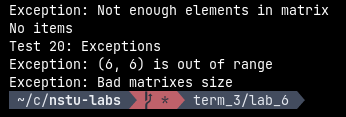
\includegraphics[width=0.5\textwidth]{lab6-test}\label{fig:lab6-test}\caption{Вывод работы программы.}\end{figure}

  \subsection{Исходный код}
  \begin{longlisting}\caption{main.cpp}\inputminted{cpp}{../../lab_6/main.cpp}\label{lst:main-cpp6}\end{longlisting}
  \begin{longlisting}\caption{matrix.hpp}\inputminted{cpp}{../../lab_6/matrix.hpp}\label{lst:matrix-hpp6}\end{longlisting}
  \begin{longlisting}\caption{matrix.cpp}\inputminted{cpp}{../../lab_6/matrix.cpp}\label{lst:matrix-cpp6}\end{longlisting}
  \begin{longlisting}\caption{file.hpp}\inputminted{cpp}{../../lab_6/file.hpp}\label{lst:file-hpp6}\end{longlisting}
  \begin{longlisting}\caption{file.cpp}\inputminted{cpp}{../../lab_6/file.cpp}\label{lst:file-cpp6}\end{longlisting}
  \begin{longlisting}\caption{circularqueue.hpp}\inputminted{cpp}{../../lab_6/circularqueue.hpp}\label{lst:circularqueue-hpp6}\end{longlisting}
  \begin{longlisting}\caption{circularqueue.cpp}\inputminted{cpp}{../../lab_6/circularqueue.cpp}\label{lst:circularqueue-cpp6}\end{longlisting}

  \subsection{Выводы}
  \par В лабораторной работе было произведена реализация механизмов работы с исключениями -- инструментами передачи управления вверх по стеку, с вызовом деструкторов объектов, расположенных на стеке. Этот механизм важен в разработке программных продуктов на языке c++, т.к. позволяет упростить код и являясь аналогом goto, быть безопасным из-за того, что исключения ``разворачивают'' стек вызывая деструкторы.

% \section{Скорость работы структуры данных}
% \begin{tikzpicture}
%   \begin{axis}[
%     y label style={at={(axis description cs:-0.05,.5)}},
%     xlabel={$n$},
%     ylabel={$t$, мс},
%     xmin=0, xmax=100000,
%     ymin=0, ymax=5500,
%     ymajorgrids=true,
%     grid style=dashed,
%     width=0.8\textwidth,
% ]

% \addplot[color=blue,mark=square]coordinates{(10000, 505.777)
% (20000, 1074.08)
% (30000, 1453.15)
% (40000, 2275.81)
% (50000, 2621.96)
% (60000, 3025.18)
% (70000, 4361.79)
% (80000, 4775.68)
% (90000, 5342.96)
% };
% \end{axis}
% \end{tikzpicture}


  \newpage
  \section*{Заключение}\label{sec:end}\addcontentsline{toc}{section}{\nameref{sec:end}}
  \par В ходе выполнения лабораторных работ была изучена система пользовательских типов языка, перегрузка операторов, виртуальные функции, исключения. Все эти языковые конструкции являются частью реализации стандартного объектно-ориентированного подхода к разработке программного обеспечения на языке c++.


  % \section*{Приложения}\label{sec:application}\addcontentsline{toc}{section}{\nameref{sec:application}}
  % \subsection*{Листинг программы}\label{sec:application1}\addcontentsline{toc}{section}{\nameref{sec:application1}}


  % \begin{longlisting}\caption{main.cpp}\inputminted{cpp}{../../lab_6/main.cpp}\label{lst:main-cpp}\end{longlisting}
  % \begin{longlisting}\caption{matrix.hpp}\inputminted{cpp}{../../lab_6/matrix.hpp}\label{lst:matrix-hpp}\end{longlisting}
  % \begin{longlisting}\caption{matrix.cpp}\inputminted{cpp}{../../lab_6/matrix.cpp}\label{lst:matrix-cpp}\end{longlisting}
  % \begin{longlisting}\caption{file.hpp}\inputminted{cpp}{../../lab_6/file.hpp}\label{lst:file-hpp}\end{longlisting}
  % \begin{longlisting}\caption{file.cpp}\inputminted{cpp}{../../lab_6/file.cpp}\label{lst:file-cpp}\end{longlisting}
  % \begin{longlisting}\caption{circularqueue.hpp}\inputminted{cpp}{../../lab_6/circularqueue.hpp}\label{lst:circularqueue-hpp}\end{longlisting}
  % \begin{longlisting}\caption{circularqueue.cpp}\inputminted{cpp}{../../lab_6/circularqueue.cpp}\label{lst:circularqueue-cpp}\end{longlisting}

\end{document}
